% Options for packages loaded elsewhere
\PassOptionsToPackage{unicode}{hyperref}
\PassOptionsToPackage{hyphens}{url}
\PassOptionsToPackage{dvipsnames,svgnames,x11names}{xcolor}
%
\documentclass[
  letterpaper,
  DIV=11,
  numbers=noendperiod]{scrreprt}

\usepackage{amsmath,amssymb}
\usepackage{iftex}
\ifPDFTeX
  \usepackage[T1]{fontenc}
  \usepackage[utf8]{inputenc}
  \usepackage{textcomp} % provide euro and other symbols
\else % if luatex or xetex
  \usepackage{unicode-math}
  \defaultfontfeatures{Scale=MatchLowercase}
  \defaultfontfeatures[\rmfamily]{Ligatures=TeX,Scale=1}
\fi
\usepackage{lmodern}
\ifPDFTeX\else  
    % xetex/luatex font selection
\fi
% Use upquote if available, for straight quotes in verbatim environments
\IfFileExists{upquote.sty}{\usepackage{upquote}}{}
\IfFileExists{microtype.sty}{% use microtype if available
  \usepackage[]{microtype}
  \UseMicrotypeSet[protrusion]{basicmath} % disable protrusion for tt fonts
}{}
\makeatletter
\@ifundefined{KOMAClassName}{% if non-KOMA class
  \IfFileExists{parskip.sty}{%
    \usepackage{parskip}
  }{% else
    \setlength{\parindent}{0pt}
    \setlength{\parskip}{6pt plus 2pt minus 1pt}}
}{% if KOMA class
  \KOMAoptions{parskip=half}}
\makeatother
\usepackage{xcolor}
\setlength{\emergencystretch}{3em} % prevent overfull lines
\setcounter{secnumdepth}{5}
% Make \paragraph and \subparagraph free-standing
\ifx\paragraph\undefined\else
  \let\oldparagraph\paragraph
  \renewcommand{\paragraph}[1]{\oldparagraph{#1}\mbox{}}
\fi
\ifx\subparagraph\undefined\else
  \let\oldsubparagraph\subparagraph
  \renewcommand{\subparagraph}[1]{\oldsubparagraph{#1}\mbox{}}
\fi


\providecommand{\tightlist}{%
  \setlength{\itemsep}{0pt}\setlength{\parskip}{0pt}}\usepackage{longtable,booktabs,array}
\usepackage{calc} % for calculating minipage widths
% Correct order of tables after \paragraph or \subparagraph
\usepackage{etoolbox}
\makeatletter
\patchcmd\longtable{\par}{\if@noskipsec\mbox{}\fi\par}{}{}
\makeatother
% Allow footnotes in longtable head/foot
\IfFileExists{footnotehyper.sty}{\usepackage{footnotehyper}}{\usepackage{footnote}}
\makesavenoteenv{longtable}
\usepackage{graphicx}
\makeatletter
\def\maxwidth{\ifdim\Gin@nat@width>\linewidth\linewidth\else\Gin@nat@width\fi}
\def\maxheight{\ifdim\Gin@nat@height>\textheight\textheight\else\Gin@nat@height\fi}
\makeatother
% Scale images if necessary, so that they will not overflow the page
% margins by default, and it is still possible to overwrite the defaults
% using explicit options in \includegraphics[width, height, ...]{}
\setkeys{Gin}{width=\maxwidth,height=\maxheight,keepaspectratio}
% Set default figure placement to htbp
\makeatletter
\def\fps@figure{htbp}
\makeatother
% definitions for citeproc citations
\NewDocumentCommand\citeproctext{}{}
\NewDocumentCommand\citeproc{mm}{%
  \begingroup\def\citeproctext{#2}\cite{#1}\endgroup}
\makeatletter
 % allow citations to break across lines
 \let\@cite@ofmt\@firstofone
 % avoid brackets around text for \cite:
 \def\@biblabel#1{}
 \def\@cite#1#2{{#1\if@tempswa , #2\fi}}
\makeatother
\newlength{\cslhangindent}
\setlength{\cslhangindent}{1.5em}
\newlength{\csllabelwidth}
\setlength{\csllabelwidth}{3em}
\newenvironment{CSLReferences}[2] % #1 hanging-indent, #2 entry-spacing
 {\begin{list}{}{%
  \setlength{\itemindent}{0pt}
  \setlength{\leftmargin}{0pt}
  \setlength{\parsep}{0pt}
  % turn on hanging indent if param 1 is 1
  \ifodd #1
   \setlength{\leftmargin}{\cslhangindent}
   \setlength{\itemindent}{-1\cslhangindent}
  \fi
  % set entry spacing
  \setlength{\itemsep}{#2\baselineskip}}}
 {\end{list}}
\usepackage{calc}
\newcommand{\CSLBlock}[1]{\hfill\break\parbox[t]{\linewidth}{\strut\ignorespaces#1\strut}}
\newcommand{\CSLLeftMargin}[1]{\parbox[t]{\csllabelwidth}{\strut#1\strut}}
\newcommand{\CSLRightInline}[1]{\parbox[t]{\linewidth - \csllabelwidth}{\strut#1\strut}}
\newcommand{\CSLIndent}[1]{\hspace{\cslhangindent}#1}

\usepackage{graphicx,float}
\usepackage{eso-pic}
\usepackage{amsmath}
\usepackage{array}      % para o \begin{array} usado pelo \stackunder
% \usepackage{stackengine} % (opcional) se quiser usar a versão do pacote \stackunder

% suas macros
\newcommand{\tn}{\mbox{\boldmath $\theta$} }
\newcommand{\sn}{\mbox{\boldmath $\sigma$} }
\newcommand{\On}{\mbox{\boldmath $\Omega$} }
\newcommand{\Dn}{\mbox{\boldmath $\Delta$} }
\newcommand{\In}{\mbox{\textbf{I}} }
\newcommand{\yn}{\mbox{\textbf{y}} }
\newcommand{\Vn}{\mbox{\textbf{V}} }
\newcommand{\mn}{\mbox{\boldmath $\mu$} }
\newcommand{\Fn}{\mbox{\boldmath $\Phi$} }
\newcommand{\Pn}{\mbox{\boldmath $\Pi$} }

\newenvironment{Dproof}[1][DProof]{\textbf{#1.} }{\ \rule{0.2cm}{0.2cm}} 
\newcommand{\stackunder}[2]{ \renewcommand{\arraystretch}{0.2} 
\displaystyle \begin{array}[t]{c}  {#1}\\_{#2}\end{array} 
\renewcommand{\arraystretch}{1}} 
\newcommand{\vect}[1]{\!\!\!\stackunder{#1}{\sim}\!\!\!}
\renewcommand{\Re}{I \! \! R}
\newcommand{\real}{\mbox{$I\!\!R$}}
\newcommand{\bi}{\begin{itemize}}
\newcommand{\ei}{\end{itemize}}
\newcommand{\va}{$X_1,\,X_2,\,\dots,\,X_n$}
\newcommand{\vam}{$x_1,\,x_2\,\ldots,\,x_n$}
\KOMAoption{captions}{tableheading}
\makeatletter
\@ifpackageloaded{tcolorbox}{}{\usepackage[skins,breakable]{tcolorbox}}
\@ifpackageloaded{fontawesome5}{}{\usepackage{fontawesome5}}
\definecolor{quarto-callout-color}{HTML}{909090}
\definecolor{quarto-callout-note-color}{HTML}{0758E5}
\definecolor{quarto-callout-important-color}{HTML}{CC1914}
\definecolor{quarto-callout-warning-color}{HTML}{EB9113}
\definecolor{quarto-callout-tip-color}{HTML}{00A047}
\definecolor{quarto-callout-caution-color}{HTML}{FC5300}
\definecolor{quarto-callout-color-frame}{HTML}{acacac}
\definecolor{quarto-callout-note-color-frame}{HTML}{4582ec}
\definecolor{quarto-callout-important-color-frame}{HTML}{d9534f}
\definecolor{quarto-callout-warning-color-frame}{HTML}{f0ad4e}
\definecolor{quarto-callout-tip-color-frame}{HTML}{02b875}
\definecolor{quarto-callout-caution-color-frame}{HTML}{fd7e14}
\makeatother
\makeatletter
\@ifpackageloaded{bookmark}{}{\usepackage{bookmark}}
\makeatother
\makeatletter
\@ifpackageloaded{caption}{}{\usepackage{caption}}
\AtBeginDocument{%
\ifdefined\contentsname
  \renewcommand*\contentsname{Índice}
\else
  \newcommand\contentsname{Índice}
\fi
\ifdefined\listfigurename
  \renewcommand*\listfigurename{Lista de Figuras}
\else
  \newcommand\listfigurename{Lista de Figuras}
\fi
\ifdefined\listtablename
  \renewcommand*\listtablename{Lista de Tabelas}
\else
  \newcommand\listtablename{Lista de Tabelas}
\fi
\ifdefined\figurename
  \renewcommand*\figurename{Figura}
\else
  \newcommand\figurename{Figura}
\fi
\ifdefined\tablename
  \renewcommand*\tablename{Tabela}
\else
  \newcommand\tablename{Tabela}
\fi
}
\@ifpackageloaded{float}{}{\usepackage{float}}
\floatstyle{ruled}
\@ifundefined{c@chapter}{\newfloat{codelisting}{h}{lop}}{\newfloat{codelisting}{h}{lop}[chapter]}
\floatname{codelisting}{Listagem}
\newcommand*\listoflistings{\listof{codelisting}{Lista de Listagens}}
\makeatother
\makeatletter
\makeatother
\makeatletter
\@ifpackageloaded{caption}{}{\usepackage{caption}}
\@ifpackageloaded{subcaption}{}{\usepackage{subcaption}}
\makeatother
\ifLuaTeX
\usepackage[bidi=basic]{babel}
\else
\usepackage[bidi=default]{babel}
\fi
\babelprovide[main,import]{brazilian}
% get rid of language-specific shorthands (see #6817):
\let\LanguageShortHands\languageshorthands
\def\languageshorthands#1{}
\ifLuaTeX
  \usepackage{selnolig}  % disable illegal ligatures
\fi
\usepackage{bookmark}

\IfFileExists{xurl.sty}{\usepackage{xurl}}{} % add URL line breaks if available
\urlstyle{same} % disable monospaced font for URLs
\hypersetup{
  pdflang={pt-br},
  colorlinks=true,
  linkcolor={blue},
  filecolor={Maroon},
  citecolor={Blue},
  urlcolor={Blue},
  pdfcreator={LaTeX via pandoc}}

\author{}
\date{}

\begin{document}

% Capa sem número
\pagenumbering{gobble}

\begin{titlepage}
\thispagestyle{empty}

% Imagem como fundo, ancorada no topo-esquerdo, sem distorção
\AddToShipoutPictureBG*{%
  \AtPageUpperLeft{%
    % "desce" a origem para dentro da página
    \raisebox{-\paperheight}{%
      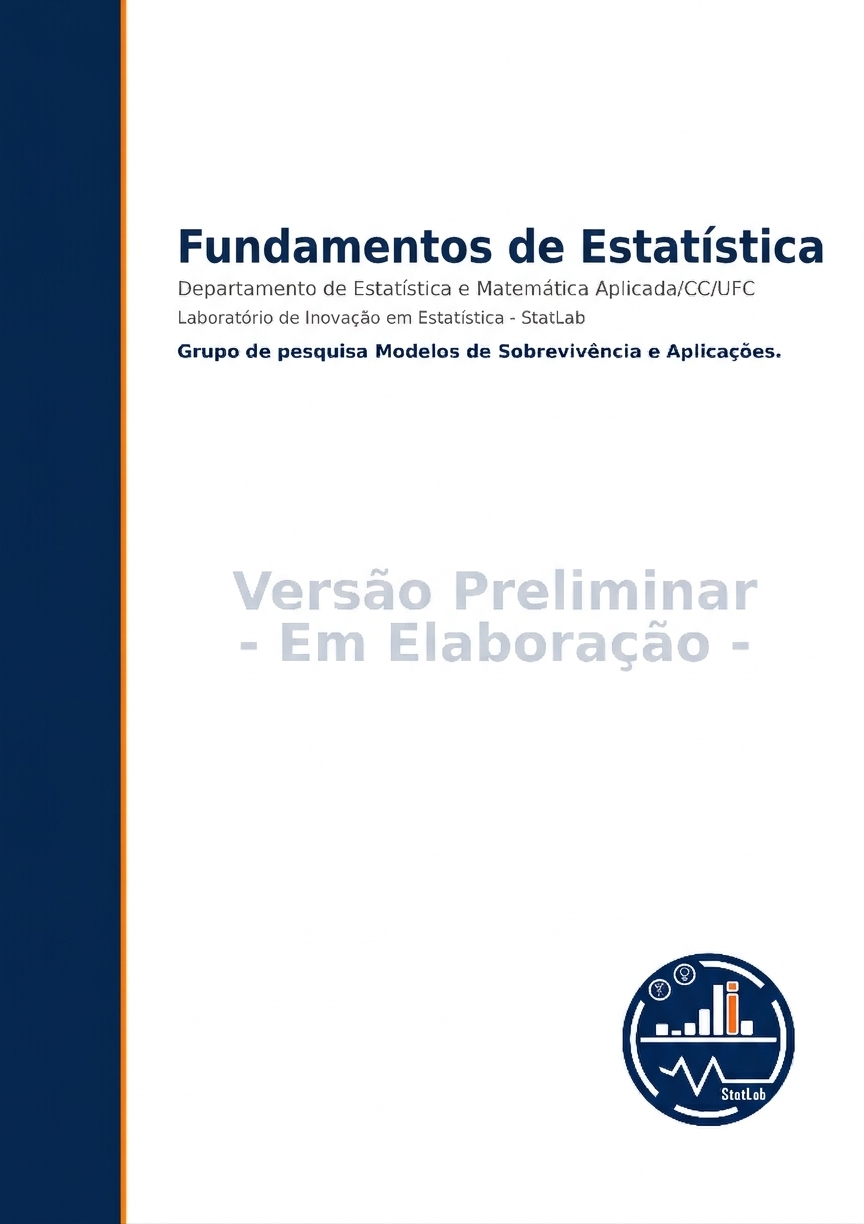
\includegraphics[width=\paperwidth,keepaspectratio]{capa.png}%
    }%
  }%
}

\null
\vfill
\end{titlepage}

\ClearShipoutPictureBG

% Reinicia numeração normal no conteúdo
\clearpage
\pagenumbering{arabic}
\setcounter{page}{1}

\renewcommand*\contentsname{Índice}
{
\hypersetup{linkcolor=}
\setcounter{tocdepth}{2}
\tableofcontents
}
\bookmarksetup{startatroot}

\chapter*{Informações Legais e Declaração de Uso de Inteligência
Artificial}\label{informauxe7uxf5es-legais-e-declarauxe7uxe3o-de-uso-de-inteliguxeancia-artificial}
\addcontentsline{toc}{chapter}{Informações Legais e Declaração de Uso de
Inteligência Artificial}

\markboth{Informações Legais e Declaração de Uso de Inteligência
Artificial}{Informações Legais e Declaração de Uso de Inteligência
Artificial}

\section*{Direitos Autorais e Uso da
Obra}\label{direitos-autorais-e-uso-da-obra}
\addcontentsline{toc}{section}{Direitos Autorais e Uso da Obra}

\markright{Direitos Autorais e Uso da Obra}

© 2026 --- Os autores.

Todos os direitos reservados. Esta obra é protegida pela legislação
brasileira de direitos autorais (Lei nº 9.610/1998). É vedada a
reprodução, distribuição, armazenamento ou transmissão total ou parcial
deste livro, por qualquer meio ou processo, eletrônico ou mecânico, sem
autorização expressa e por escrito dos autores, salvo nos casos
permitidos pela legislação vigente para fins exclusivamente acadêmicos e
não comerciais, com a devida citação da fonte.

A utilização do material em ambientes de ensino é permitida desde que
preservada a integridade do conteúdo, mencionada a autoria e respeitados
os princípios de uso responsável da informação científica. A reprodução
para fins comerciais, bem como a modificação substancial do conteúdo sem
autorização, constitui violação de direitos autorais.

\section*{Declaração sobre o Uso de Ferramentas de Inteligência
Artificial}\label{declarauxe7uxe3o-sobre-o-uso-de-ferramentas-de-inteliguxeancia-artificial}
\addcontentsline{toc}{section}{Declaração sobre o Uso de Ferramentas de
Inteligência Artificial}

\markright{Declaração sobre o Uso de Ferramentas de Inteligência
Artificial}

Durante a elaboração deste livro foram utilizadas ferramentas de
Inteligência Artificial, em especial sistemas de apoio à escrita e
organização textual, como recurso complementar no processo de produção
acadêmica.

O uso de IA teve caráter \textbf{estritamente assistivo}, não
substituindo o desenvolvimento conceitual, a formulação matemática, a
interpretação estatística nem as decisões pedagógicas da obra. Todo
conteúdo foi cuidadosamente revisado, validado e adaptado pelos autores,
que assumem integral responsabilidade científica e intelectual pelo
texto final.

Não foram delegadas à IA decisões metodológicas, inferenciais ou
conclusões analíticas. A elaboração teórica, a seleção de exemplos, a
validação matemática e a coerência didática resultam da experiência
acadêmica e da atuação dos autores na área de Modelos de Regressão.

Reafirmamos que o uso responsável de tecnologias emergentes deve sempre
preservar o rigor científico, a integridade acadêmica e o protagonismo
intelectual humano.

\bookmarksetup{startatroot}

\chapter*{Prefácio}\label{prefuxe1cio}
\addcontentsline{toc}{chapter}{Prefácio}

\markboth{Prefácio}{Prefácio}

Este livro resulta da experiência acumulada no ensino, na orientação de
estudantes e no desenvolvimento de pesquisas em modelos de regressão.
Somos docentes pesquisadores do Departamento de Estatística e Matemática
Aplicada da Universidade Federal do Ceará (DEMA/UFC), com atuação
contínua em regressão linear, modelagem estatística e inferência.
Integramos o Laboratório de Inovação em Estatística --- StatLab/UFC
(\url{https://statlab.quarto.pub/}) e o Grupo de Pesquisa \emph{Modelos
de Sobrevivência e Aplicações} do CNPq
(\url{http://dgp.cnpq.br/dgp/espelhogrupo/9639095385610769}), espaços
nos quais articulamos ensino, pesquisa e aplicação a problemas reais.

O material tem como base as disciplinas Inferência Estatística I
(CC0288) e Análise Inferencial (CC0448). Ao longo dos anos, consolidamos
a convicção de que ensinar regressão exige equilíbrio entre rigor
teórico e clareza interpretativa.

O livro desenvolve os conceitos de introdutórios de Estatística de forma
progressiva, enfatizando interpretação e propriedades. A implementação é
realizada integralmente no \textbf{R}, utilizado como ambiente de
experimentação conceitual e não apenas como ferramenta computacional.

Os fundamentos matemáticos mais densos são apresentados em apêndices
específicos, preservando o fluxo didático do texto principal e
permitindo diferentes níveis de aprofundamento. Acreditamos que
inferência deve ser ensinada como base para tomada de decisão, com
atenção às suas suposições, limitações e implicações práticas.

Esperamos que este livro contribua para a formação de profissionais
capazes tomar decisões com rigor técnico, pensamento estatístico crítico
e responsabilidade analítica.

\bookmarksetup{startatroot}

\chapter{Introdução}\label{introduuxe7uxe3o}

A origem da palavra \textbf{Estatística} está associada à palavra latina
STATUS (Estado). Há indícios de que 3000 anos A.C. já se faziam
\emph{censos na Babilônia}, China e Egito e até mesmo o 4º livro do
\emph{Velho Testamento} faz referência à uma instrução dada a Moisés,
para que fizesse um levantamento dos homens de Israel que estivessem
aptos para guerrear. Usualmente, estas informações eram utilizadas para
a \emph{taxação de impostos} ou para o \emph{alistamento militar}. O
Imperador \emph{César Augusto}, por exemplo, ordenou que se fizesse o
Censo de todo o Império Romano.

A palavra \textbf{CENSO} é derivada da palavra \emph{CENSERE}, que em
Latim significa \emph{TAXAR}. Em 1085, \emph{Guilherme, O Conquistador},
solicitou um levantamento estatístico da Inglaterra, que deveria conter
informações sobre terras, proprietários, uso da terra, empregados e
animais. Os resultados deste censo foram publicados em 1086 no livro
intitulado \emph{``Domesday Book''} e serviram de base para o
\emph{cálculo de impostos}.

Contudo, mesmo que a prática de coletar dados sobre colheitas,
composição da população humana ou de animais, impostos, etc., fosse
conhecida pelos egípcios, hebreus, caldeus e gregos, e se atribuam a
Aristóteles cento e oitenta descrições de Estados, apenas no
\emph{século XVII} a Estatística passou a ser considerada
\emph{disciplina autônoma}, tendo como objetivo básico a \emph{descrição
dos BENS do Estado}.

A palavra \textbf{Estatística} foi cunhada pelo acadêmico alemão
\emph{Gottfried Achenwall} (1719-1772), que foi um notável continuador
dos estudos de \emph{Hermann Conrig} (1606-1681). A escola alemã atingiu
sua maturidade com \emph{A. L. Von Schlozer} (1735-1809), mas sempre com
ideias diferentes daquelas que fundamentaram a Estatística Moderna. Com
algum exagero, pode-se dizer que o seu principal legado foi o termo
\emph{STAATENKUNDE}, que deu origem à designação atual. Na Enciclopédia
Britânica, o verbete \emph{STATISTICS} apareceu em 1797.

Em contraposição à natureza eminentemente qualitativa da escola alemã,
na Inglaterra do século XVII surgiram os aritméticos políticos, dentre
os quais se destacaram \emph{John Graunt} (1620-1674) e \emph{William
Petty} (1623-1687). Eles preocuparam-se com o estudo numérico dos
fenômenos sociais e políticos, na busca de leis quantitativas que
pudessem explicá-los. O estudo consistia essencialmente de exaustivas
análises de nascimentos e mortes, realizadas através das \emph{Tábuas de
Mortalidade}, que deram origem às atuais tábuas usadas pelas companhias
de seguros. Dessa forma, a escola dos aritméticos políticos pode ser
considerada o berço da \emph{Demografia}. Um de seus mais notáveis
adeptos foi o pastor alemão \emph{Sussmilch} (1707-1767), com o qual
pode-se dizer que a Estatística aparece pela primeira vez como meio
indutivo de investigação.

Na última metade do século XIX, os alemães \emph{Helmert} (1843-1917) e
\emph{Wilhelm Lexis} (1837-1914), o dinamarquês \emph{Thorvald Nicolai
Thiele} (1838-1910) e o inglês \emph{Francis Ysidro Edgeworth}
(1845-1926), obtiveram resultados extremamente valiosos para o
desenvolvimento da Inferência Estatística, muitos dos quais só foram
completamente compreendidos mais tarde. Contudo, o impulso decisivo
deve-se a \emph{Karl Pearson} (1857-1936), \emph{William S. Gosset}
(1876-1937) e, em especial, a \emph{Ronald A. Fisher} (1890-1962).

\section{Figuras ilustres na área de
Estatística}\label{figuras-ilustres-na-uxe1rea-de-estatuxedstica}

\begin{figure}

\begin{minipage}{\linewidth}

\begin{figure}[H]

\centering{

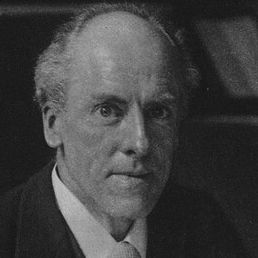
\includegraphics[width=0.86in,height=\textheight]{pearson.png}

}

\caption{\label{fig-pearson}Karl Pearson}

\end{figure}%

\end{minipage}%

\end{figure}%

\href{https://www.britannica.com/biography/Karl-Pearson}{Karl Pearson}
(1857-1936) formou-se em 1879 pela Cambridge University e inicialmente
dedicou-se ao estudo da evolução de Darwin, aplicando os métodos
estatísticos aos problemas biológicos relacionados com a evolução e
hereditariedade. Em 1896, Pearson foi eleito membro da Royal Society of
London. Entre 1893 e 1912 escreveu um conjunto de 18 artigos denominado
Mathematical Contribution to the Theory Evolution, com contribuições
extremamente importantes para o desenvolvimento da teoria da Análise de
Regressão e do Coeficiente de Correlação, bem como do Teste de Hipóteses
de Qui-quadrado. Em sua maioria, seus trabalhos foram publicados na
revista Biometrika, que fundou em parceria com \textbf{Walter Frank
Raphael Weldon} (1860-1906) e \textbf{Francis Galton} (1822-1911). Além
da valiosa contribuição que deu para a teoria da regressão e da
correlação, Pearson fez com que a Estatística fosse reconhecida como uma
disciplina autônoma. Uma coleção de seus artigos foi publicada em
\emph{``Karl Pearson Early Statistical Papers'' (Ed. por E. S. Pearson,
Cambridge University Press, 1948)}.

\begin{figure}

\begin{minipage}{\linewidth}

\begin{figure}[H]

\centering{

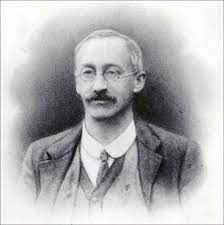
\includegraphics[width=0.75in,height=\textheight]{gosset.png}

}

\caption{\label{fig-gosset}William Sealey Gosset}

\end{figure}%

\end{minipage}%

\end{figure}%

\href{https://rss.onlinelibrary.wiley.com/doi/10.1111/j.1740-9713.2008.00279.x}{William
Sealey Gosset} (1876-1937) estudou Química e Matemática na \emph{New
College Oxford}. Em 1899 foi contratado como Químico da Cervejaria
Guiness em Dublin, desenvolvendo um trabalho extremamente importante na
área de Estatística. Devido à necessidade de manipular dados
provenientes de pequenas amostras, extraídas para melhorar a qualidade
da cerveja, Gosset derivou o teste t de Student baseado na distribuição
de probabilidades. Esses resultados foram publicados em 1908 na revista
\emph{Biometrika}, sob o pseudônimo de Student, dando origem a uma nova
e importante fase dos estudos estatísticos. \textbf{Gosset} usava o
pseudônimo de \textbf{Student}, pois a Cervejaria Guiness não desejava
revelar aos concorrentes os métodos estatísticos que estava empregando
no controle de qualidade da cerveja. Os estudos de \textbf{Gosset} podem
ser encontrados em \emph{``Student Collected Papers'' (Ed. por
E.S.Pearson e J. Wishart, University College, Londres, 1942)}.

\begin{figure}

\begin{minipage}{\linewidth}

\begin{figure}[H]

\centering{

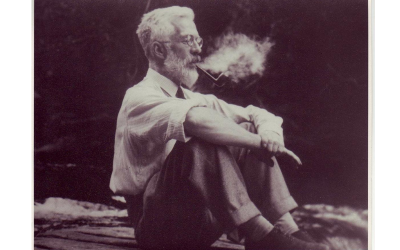
\includegraphics[width=1.33in,height=\textheight]{Fisher.png}

}

\caption{\label{fig-fisher}Ronald Aylmer Fisher}

\end{figure}%

\end{minipage}%

\end{figure}%

A contribuição de
\href{https://www.ucl.ac.uk/biosciences/gee/ucl-centre-computational-biology/ronald-aylmer-fisher-1890-1962}{Ronald
Aylmer Fisher} (1890-1962) para a Estatística Moderna é, sem dúvidas, a
mais importante e decisiva de todas. Formado em astronomia pela
Universidade de Cambridge em 1912, foi o fundador do célebre Statistical
Laboratory da prestigiosa Estação Agronômica de Rothamsted, contribuindo
enormemente tanto para o desenvolvimento da Estatística quanto da
Genética. Ele apresentou os princípios de Planejamento de Experimentos,
introduzindo os conceitos de Aleatorização e da Análise da Variância,
procedimentos muito usados atualmente.

No princípio dos \textbf{anos 20}, estabeleceu o que a maioria aceita
como a estrutura da moderna Estatística Analítica, através do conceito
da verossimilhança (likelihood). O seu livro intitulado ``Statistical
Methods for Research Workers'', publicado pela primeira vez em 1925, foi
extremamente importante para familiarizar os investigadores com as
aplicações práticas dos métodos estatísticos e, também, para criar a
mentalidade estatística entre a nova geração de cientistas.

Os trabalhos de \textbf{Fisher} encontram-se dispersos em numerosas
revistas, mas suas contribuições mais importantes foram reunidas em
\emph{``Contributions to Mathematical Statistics'' (J. Wiley \& Sons,
Inc.,Nova Iorque, 1950)}. Fisher foi eleito membro da \emph{Royal
Society} em 1929 e condecorado com as medalhas \emph{Royal Medal of the
Society} em 1938 e \emph{Darwin Medal of the Society} em 1948. Em 1955
foi novamente condecorado, desta vez com a medalha \emph{Copley Medal of
the Royal Society}.

\begin{figure}

\begin{minipage}{\linewidth}

\begin{figure}[H]

\centering{

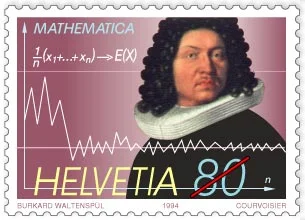
\includegraphics[width=1.02in,height=\textheight]{Jakob.png}

}

\caption{\label{fig-bernoulli}Jakob Bernoulli}

\end{figure}%

\end{minipage}%

\end{figure}%

\href{https://www.britannica.com/biography/Jakob-Bernoulli}{Jakob
Bernoulli} (1654-1705), estimulado por \emph{Gottfried Wilhelm von
Leibniz} (1646-1716) também dedicou-se ao estudo do Cálculo de
Probabilidades, cuja grande obra denominada \emph{``Ars Conjectandi''}
foi publicada oito anos após a sua morte. Em \emph{Ars Conjectandi} de
\textbf{Jacques Bernoulli}, foi rigorosamente provada a Lei dos Grandes
Números de Bernoulli, considerada o primeiro teorema limite. Pode-se
dizer que graças às contribuições de \textbf{Bernoulli} o Cálculo de
Probabilidades adquiriu o status de ciência. Além da obra póstuma de
\textbf{Bernoulli}, o início do século XVII foi marcado pelos livros de
\emph{Pierre Rémond de Montmort} (1678-1719), denominado \emph{``Essai
d'Analyse sur les Jeux de Hazard''}, e de \emph{Abraham De Moivre}
(1667-1754), intitulado \emph{``The Doctrine of Chances''}.

\begin{figure}

\begin{minipage}{\linewidth}

\begin{figure}[H]

\centering{

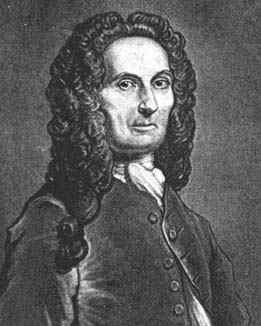
\includegraphics[width=0.87in,height=\textheight]{Moivre.png}

}

\caption{\label{fig-moivre}Abraham de Moivre}

\end{figure}%

\end{minipage}%

\end{figure}%

\href{https://www.britannica.com/biography/Abraham-de-Moivre}{Abraham de
Moivre} era Francês de nascimento, mas desde a sua infância refugiou-se
na Inglaterra devido às guerras religiosas, fazendo aplicações ao
cálculo de anuidades e estabelecendo uma equação simples para a lei da
mortalidade entre 22 anos e o limite da longevidade que fixou em 86
anos. Mais tarde, na \emph{``Miscellanea Analytica''}, apresentou
resultados aos quais \textbf{Laplace} deu uma forma mais geral e que
constituem o \emph{segundo teorema limite}. Em 1738, com a segunda
edição da \emph{Doutrina das Chances (The Doctrine of Chances)}, publica
formalmente a Distribuição Normal, desenvolvida desde 1933.

\begin{figure}

\begin{minipage}{\linewidth}

\begin{figure}[H]

\centering{


\includegraphics[width=2.67in,height=\textheight]{Bayes.png}

}

\caption{\label{fig-bayes}Thomas Bayes}

\end{figure}%

\end{minipage}%

\end{figure}%

É extremamente importante falar, também, do reverendo
\href{https://www.britannica.com/topic/Nonconformist}{Thomas Bayes}
(1702-1761) a quem se deve o conceito de probabilidade inversa,
relacionado com situações em que se caminha do particular para o geral.
No seu livro denominado \emph{``Essay towards solving a problem of the
doctrine of chances'' (Philosophical Transactions of the Royal Society
of London, 1764-65, póstumo)}, \textbf{Bayes} formula através do teorema
que leva seu nome e do postulado que tantas vezes se lhe associa: a
primeira tentativa de matematização da inferência Estatística. Mesmo sem
ter publicado nenhum trabalho com seu nome, em 1742 \textbf{Thomas
Bayes} foi eleito membro da \emph{Royal Society of London}.

\begin{figure}

\begin{minipage}{\linewidth}

\begin{figure}[H]

\centering{

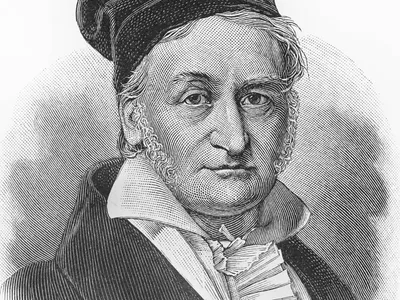
\includegraphics[width=1.33in,height=\textheight]{Gauss.png}

}

\caption{\label{fig-gauss}Johann Carl Friedrich Gauss}

\end{figure}%

\end{minipage}%

\end{figure}%

Os estudos dos astrônomos Pierre-Simon Laplace (1749-1827),
\href{https://www.britannica.com/biography/Carl-Friedrich-Gauss}{Johann
Carl Friedrich Gauss} (1777-1855) e \emph{Lambert Adolphe Jacques
Quetelet} (1796-1874) foram fundamentais para o desenvolvimento do
Cálculo de Probabilidades. Devido aos novos métodos e idéias, o trabalho
de \emph{Laplace} de 1812, intitulado \emph{``Théorie Analytique des
Probabilités''}, até o presente é considerado um dos mais importantes
trabalhos sobre a matéria. \textbf{Johann Carl Friedrich Gauss},
professor de astronomia e diretor do Observatório de Gottingen, em 1809
apresentou o estudo intitulado \emph{``Theoria combinationis
Observatorium Erroribus Minimis Obnoxia''}, explanando uma teoria sobre
a análise de observações aplicável a qualquer ramo da ciência, alargando
o campo de aplicação do Cálculo de Probabilidades. Com \emph{Lambert
Adolphe Jacques Quetelet}, por sua vez, inicia-se a aplicação aos
fenômenos sociais. O seu escrito \emph{``Sur l'homme et le développement
de ses facultes''} foi publicado em segunda edição com o título
\emph{``Physique sociale''} ou \emph{``Essai sur le développement des
facultés de l'homme''}, que incluía pormenorizada análise da teoria da
probabilidade. \emph{Quetelet} introduziu também o conceito de ``homem
médio'' e chamou particular atenção para a notável consistência dos
fenômenos sociais. Por exemplo, mostrou que fatores como a criminalidade
apresentam permanências em relação a diferentes países e classes
sociais.

\begin{figure}

\begin{minipage}{\linewidth}

\begin{figure}[H]

\centering{

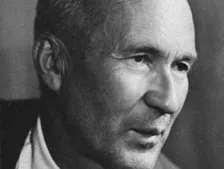
\includegraphics[width=0.75in,height=\textheight]{Kolmo.png}

}

\caption{\label{fig-kolmogorov}Andrey Nikolayevich Kolmogorov}

\end{figure}%

\end{minipage}%

\end{figure}%

Na segunda metade do século XIX a Teoria das Probabilidades atingiu um
dos pontos mais altos com os trabalhos da escola russa fundada por
\emph{Pafnuty Lvovich Chebyshev} (1821-1894), que contou com
representantes como \emph{Andrei Andreyevich Markov} (1856-1922) e
\emph{Aleksandr Mikhailovich Lyapunov} (1857-1918). Contudo, o seu maior
expoente foi
\href{https://www.britannica.com/biography/Andrey-Nikolayevich-Kolmogorov}{Andrey
Nikolayevich Kolmogorov} (1903-1987), a quem se deve um estudo
indispensável sobre os fundamentos da Teoria das Probabilidades (os
axiomas de Kolmogorov), denominado \emph{``Grundbegrife der
Warscheinlichkeitrechnung''}, publicado em 1933. Em 1950 foi traduzido
para o Inglês sob o título \emph{``Foundations of Probability''}.

\section{Atividade}\label{atividade}

\begin{enumerate}
\def\labelenumi{\arabic{enumi}.}
\tightlist
\item
  Foram destacados apenas contribuições masculinas para a área da
  Estatística. Pesquise sobre mulheres que foram importantes para o
  desenvolvimento desta área.
\end{enumerate}

\bookmarksetup{startatroot}

\chapter{Estatística Descritiva}\label{estatuxedstica-descritiva}

Fases do Método e Conceitos Iniciais

\hfill\break

\section{1. Fases do Método
Estatístico}\label{fases-do-muxe9todo-estatuxedstico}

\subsection{Métodos de Pesquisa}\label{muxe9todos-de-pesquisa}

Na pesquisa científica, o procedimento geral consiste em formular
hipóteses e testá-las. Inicialmente, essas hipóteses são formuladas em
termos científicos da área de estudo e, em seguida, expressas em termos
estatísticos.

\subsubsection{O Método Científico}\label{o-muxe9todo-cientuxedfico}

Conjunto de normas básicas para a produção de conhecimento com rigor
científico. Destacamos dois métodos:

\begin{tcolorbox}[enhanced jigsaw, colframe=quarto-callout-note-color-frame, colback=white, bottomrule=.15mm, bottomtitle=1mm, toptitle=1mm, opacitybacktitle=0.6, arc=.35mm, breakable, rightrule=.15mm, colbacktitle=quarto-callout-note-color!10!white, titlerule=0mm, leftrule=.75mm, title={Nota}, toprule=.15mm, left=2mm, opacityback=0, coltitle=black]

\textbf{Método Experimental} Consiste em manter constantes todas as
causas (fatores), menos uma, e variá-la para descobrir seus efeitos.
Comum na Física e Química. \emph{(CRESPO, 2002)}

\end{tcolorbox}

\begin{tcolorbox}[enhanced jigsaw, colframe=quarto-callout-note-color-frame, colback=white, bottomrule=.15mm, bottomtitle=1mm, toptitle=1mm, opacitybacktitle=0.6, arc=.35mm, breakable, rightrule=.15mm, colbacktitle=quarto-callout-note-color!10!white, titlerule=0mm, leftrule=.75mm, title={Nota}, toprule=.15mm, left=2mm, opacityback=0, coltitle=black]

\textbf{Método Estatístico} Admite todas as causas presentes
variando-as, registrando essas variações para determinar a influência de
cada uma. \emph{(COSTA, 2011)}

\end{tcolorbox}

\subsection{As Fases do Método
Estatístico}\label{as-fases-do-muxe9todo-estatuxedstico}

Segundo Castanheira (2003), o método divide-se em seis etapas lógicas:

\begin{enumerate}
\def\labelenumi{\arabic{enumi}.}
\tightlist
\item
  \textbf{Definição do Problema:} Saber exatamente o que se pretende
  pesquisar.
\item
  \textbf{Planejamento:} Determinar objetivos, amostra e cronograma.
\item
  \textbf{Coleta de Dados:} Obtenção das informações (Primárias ou
  Secundárias).
\item
  \textbf{Apuração dos Dados:} Resumo, contagem e tabulação.
\item
  \textbf{Apresentação dos Dados:} Exposição em tabelas ou gráficos.
\item
  \textbf{Análise e Interpretação:} Cálculo de medidas e descrição do
  fenômeno.
\end{enumerate}

\section{2. Coleta e Tipos de Dados}\label{coleta-e-tipos-de-dados}

\subsection{Formas de Coleta}\label{formas-de-coleta}

A coleta pode ser classificada quanto à sua periodicidade:

\begin{itemize}
\tightlist
\item
  \textbf{Contínua:} Registros constantes (nascimentos, óbitos).
\item
  \textbf{Periódica:} Intervalos constantes (Censos, avaliações
  mensais).
\item
  \textbf{Ocasional:} Situações emergenciais ou específicas (surto de
  dengue).
\end{itemize}

\subsection{Natureza dos Dados}\label{natureza-dos-dados}

\begin{longtable}[]{@{}
  >{\raggedright\arraybackslash}p{(\columnwidth - 4\tabcolsep) * \real{0.3333}}
  >{\raggedright\arraybackslash}p{(\columnwidth - 4\tabcolsep) * \real{0.3333}}
  >{\raggedright\arraybackslash}p{(\columnwidth - 4\tabcolsep) * \real{0.3333}}@{}}
\toprule\noalign{}
\begin{minipage}[b]{\linewidth}\raggedright
Tipo
\end{minipage} & \begin{minipage}[b]{\linewidth}\raggedright
Descrição
\end{minipage} & \begin{minipage}[b]{\linewidth}\raggedright
Fontes Comuns
\end{minipage} \\
\midrule\noalign{}
\endhead
\bottomrule\noalign{}
\endlastfoot
\textbf{Primários} & Publicados pela própria pessoa/órgão que os
recolheu. & Entrevistas, questionários. \\
\textbf{Secundários} & Publicados por outra organização (já existentes).
& IBGE, relatórios empresariais. \\
\end{longtable}

\section{3. Análise Exploratória de Dados
(AED)}\label{anuxe1lise-exploratuxf3ria-de-dados-aed}

\begin{quote}
\emph{``It is important to understand what you CAN DO, before you learn
to measure how WELL you seem to have DONE it.''} \textgreater{} ---
\textbf{John Tukey (1977)}
\end{quote}

A AED busca entender a estrutura dos dados antes da inferência. Seus
objetivos incluem: * Limpeza de dados adicional. * Identificação de
relações entre variáveis. * Sugestão de hipóteses para testes futuros.

\begin{tcolorbox}[enhanced jigsaw, colframe=quarto-callout-tip-color-frame, colback=white, bottomrule=.15mm, bottomtitle=1mm, toptitle=1mm, opacitybacktitle=0.6, arc=.35mm, breakable, rightrule=.15mm, colbacktitle=quarto-callout-tip-color!10!white, titlerule=0mm, leftrule=.75mm, title=\textcolor{quarto-callout-tip-color}{\faLightbulb}\hspace{0.5em}{Nota sobre Software}, toprule=.15mm, left=2mm, opacityback=0, coltitle=black]

A utilização de programas como o \textbf{R} é uma ferramenta
complementar. Embora o foco seja o conceito, demonstraremos como
realizar as análises de forma computacional.

\end{tcolorbox}

\section{4. Conceitos Fundamentais}\label{conceitos-fundamentais}

\begin{itemize}
\tightlist
\item
  \textbf{População:} Conjunto total de elementos com uma característica
  comum.
\item
  \textbf{Amostra:} Subconjunto representativo da população.
\item
  \textbf{Censo:} Estudo que abrange todos os elementos da população.
\end{itemize}

\subsection{Divisão da Estatística}\label{divisuxe3o-da-estatuxedstica}

\begin{enumerate}
\def\labelenumi{\arabic{enumi}.}
\tightlist
\item
  \textbf{Descritiva:} Técnicas para descrever e resumir dados (tabelas
  e gráficos).
\item
  \textbf{Inferencial:} Uso de amostras para fazer generalizações sobre
  a população.
\end{enumerate}

\section{5. Tipos de Variáveis}\label{tipos-de-variuxe1veis}

Uma \textbf{variável} é a característica de interesse que estudamos em
uma população.

\begin{figure}

\begin{minipage}{0.50\linewidth}

\subsubsection{Qualitativas (Atributos)}\label{qualitativas-atributos}

\begin{itemize}
\tightlist
\item
  \textbf{Nominal:} Sem ordem (Ex: Cor dos olhos, sexo).
\item
  \textbf{Ordinal:} Com hierarquia (Ex: Escolaridade, classe social).
\end{itemize}

\end{minipage}%
%
\begin{minipage}{0.50\linewidth}

\subsubsection{Quantitativas (Números)}\label{quantitativas-nuxfameros}

\begin{itemize}
\tightlist
\item
  \textbf{Discreta:} Contagem, valores inteiros (Ex: Nº de filhos).
\item
  \textbf{Contínua:} Medição, valores reais (Ex: Peso, altura).
\end{itemize}

\end{minipage}%

\end{figure}%

\section{📝 Exercícios de Fixação}\label{exercuxedcios-de-fixauxe7uxe3o}

Classifique as variáveis abaixo:

\begin{enumerate}
\def\labelenumi{\arabic{enumi}.}
\tightlist
\item
  Cor dos olhos de candidatos: \_\_\_\_\_\_\_\_\_\_\_\_\_\_\_\_\_\_\_\_
\item
  Número de filhos de casais: \_\_\_\_\_\_\_\_\_\_\_\_\_\_\_\_\_\_\_\_
\item
  Salários de funcionários: \_\_\_\_\_\_\_\_\_\_\_\_\_\_\_\_\_\_\_\_
\item
  Classificação em concurso público:
  \_\_\_\_\_\_\_\_\_\_\_\_\_\_\_\_\_\_\_\_
\item
  Renda de clientes de um banco:
  \_\_\_\_\_\_\_\_\_\_\_\_\_\_\_\_\_\_\_\_
\end{enumerate}

\bookmarksetup{startatroot}

\chapter{Introdução à
Probabilidade}\label{introduuxe7uxe3o-uxe0-probabilidade}

\bookmarksetup{startatroot}

\chapter{Introdução à
Inferência}\label{introduuxe7uxe3o-uxe0-inferuxeancia}

\bookmarksetup{startatroot}

\chapter{Introdução à
Regressão}\label{introduuxe7uxe3o-uxe0-regressuxe3o}

\bookmarksetup{startatroot}

\chapter*{Referências}\label{referuxeancias}
\addcontentsline{toc}{chapter}{Referências}

\markboth{Referências}{Referências}

\phantomsection\label{refs}
\begin{CSLReferences}{0}{1}
\end{CSLReferences}



\end{document}
